\documentclass[11pt,border=2pt]{standalone}
\usepackage{amsmath,amssymb}
\usepackage{xcolor}
\usepackage{tikz}
\usepackage{pgfplots}
\pgfplotsset{compat=1.18}
\usetikzlibrary{calc,arrows,positioning,fit,backgrounds,decorations.pathreplacing,patterns}
\definecolor{cElem}{RGB}{40,80,140}
\definecolor{cTrg}{RGB}{190,40,40}
\definecolor{cCell}{RGB}{225,238,248}
\definecolor{cAcc}{RGB}{240,200,120}
\definecolor{cGrey}{RGB}{120,120,120}
\definecolor{cVec}{RGB}{110,55,150}
\begin{document}
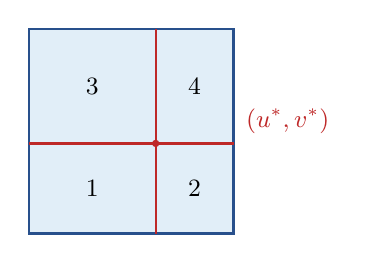
\begin{tikzpicture}[scale=2.6]
  \def\ux{0.62} \def\vy{0.44}
  \fill[cCell] (0,0) rectangle (1,1);
  \draw[cElem,thick] (0,0) rectangle (1,1);
  \draw[cTrg,thick] (\ux,0) -- (\ux,1);
  \draw[cTrg,thick] (0,\vy) -- (1,\vy);
  \fill[cTrg] (\ux,\vy) circle (0.018);
  \node[cTrg,font=\small,above right=0pt and 1pt] at (1.0,\vy) {$(u^\ast,v^\ast)$};
  \node[font=\small] at (0.31,0.22) {1};
  \node[font=\small] at (0.81,0.22) {2};
  \node[font=\small] at (0.31,0.72) {3};
  \node[font=\small] at (0.81,0.72) {4};
\end{tikzpicture}
\end{document}
